\documentclass[10pt,a4paper]{article}
\usepackage[utf8]{inputenc}
\usepackage[T1]{fontenc}
\usepackage{amsmath}
\usepackage{amssymb}
\usepackage{graphicx}
\usepackage[english]{babel}
\usepackage{url}
\usepackage{dirtree}
\usepackage{textcomp}
\usepackage{hyperref}
\usepackage{listings, lstautogobble}
\lstset{ 
	upquote=true,
	columns=fullflexible,
	basicstyle=\ttfamily,
	literate={*}{{\char42}}1
		{-}{{\char45}}1
		{\ }{{\copyablespace}}1,
	autogobble=true
}
\usepackage[space=true]{accsupp}
\newcommand{\copyablespace}{\BeginAccSupp{method=hex,unicode,ActualText=00A0}\hphantom{x}\EndAccSupp{}}

\usepackage{xcolor}

\colorlet{punct}{red!60!black}
\definecolor{background}{HTML}{EEEEEE}
\definecolor{delim}{RGB}{20,105,176}
\colorlet{numb}{magenta!60!black}

\lstdefinelanguage{json}{
	basicstyle=\normalfont\ttfamily,
	%numbers=left,
	%numberstyle=\scriptsize,
	%stepnumber=1,
	%numbersep=8pt,
	showstringspaces=false,
	breaklines=true,
	frame=lines,
	backgroundcolor=\color{background},
	literate=
	*{0}{{{\color{numb}0}}}{1}
	{1}{{{\color{numb}1}}}{1}
	{2}{{{\color{numb}2}}}{1}
	{3}{{{\color{numb}3}}}{1}
	{4}{{{\color{numb}4}}}{1}
	{5}{{{\color{numb}5}}}{1}
	{6}{{{\color{numb}6}}}{1}
	{7}{{{\color{numb}7}}}{1}
	{8}{{{\color{numb}8}}}{1}
	{9}{{{\color{numb}9}}}{1}
	{:}{{{\color{punct}{:}}}}{1}
	{,}{{{\color{punct}{,}}}}{1}
	{\{}{{{\color{delim}{\{}}}}{1}
	{\}}{{{\color{delim}{\}}}}}{1}
	{[}{{{\color{delim}{[}}}}{1}
	{]}{{{\color{delim}{]}}}}{1},
}

\title{The Hangman Game\\User Manual}
\author{}
\date{}

\begin{document}
	\maketitle
	\section{About the Game}
		The hangman game consists in trying to guess a word that is shown on screen by underscore characters or asterisks. 
		The player will know the length of the word but not the letters it is composed of.
		Each round the player will guess a character, if the character is in the word that letter will be uncovered.
		If the character is not in the word the player will lose a life. 
		The player has 6 lives, meaning that they can fail their guess a total of 6 times.
		Once the player has no lives left the game ends.
		
		At any point the player has an option for guessing the word, if the guess is correct they will win the game.
		If the guess is not correct the player will lose a life.
		
	\section{Launching the Game}
		At this point in time the game only work on Linux.
	
		The game can be downloaded from the following URL:\\ \href{https://miaulario.unavarra.es/access/content/group/2023\_0\_505108\_81\_G/Lab\%20Handouts/02.-Hangman/hangman.bin}{\url{https://miaulario.unavarra.es/access/content/group/2023\_0\_505108\_81\_G/Lab\%20Handouts/02.-Hangman/hangman.bin}}
		
		Once downloaded we will have to allow the execution of the game by executing the following command in the console:
		\begin{verbatim}
			chmod +x hangman.bin
		\end{verbatim}
		
		Then to launch it we will use the next command:
		\begin{verbatim}
			./hangman.bin
		\end{verbatim}
	
	\section{Starting}
		The game requires a JSON file that contains the words that are going to be played.
		The words will be organized into several categories, this way the structure of the file can be described as dictionary where the categories are the keys and a list of words will be the values.
		An example file can be seen on Listing~\ref{lst:json}:
		\newpage
		\begin{lstlisting}[language=json, caption={JSON file example}, captionpos=b, label=lst:json]
			{
				"transportation": [
					"scooter",
					"bicycle",
					"airplane"
				],
				"food": [
					"chicken",
					"pasta",
					"porridge",
				],
			}
		\end{lstlisting}
		
	
		Whenever the game starts it will check for the existence of a file called \texttt{words.json}. 
		If this file does not exist it will ask the user if it wants to create one.
		\begin{figure}[hbtp]
			\centering
			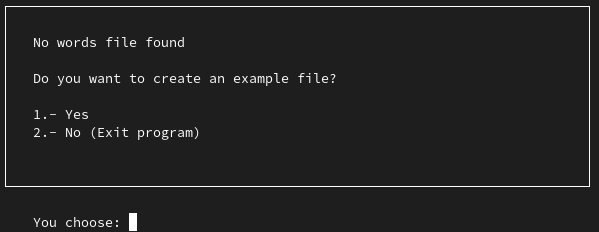
\includegraphics[width=0.7\linewidth]{img/create_words}
			\caption{If the words file is not found the game will show this menu}
			\label{fig:createwords}
		\end{figure}
		
		If the program finds a \texttt{words.json} file or one is created the main menu will be shown.
		
		\begin{figure}[hbtp]
			\centering
			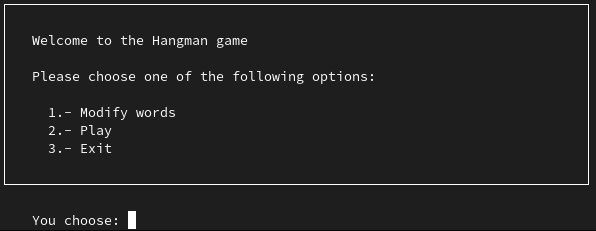
\includegraphics[width=0.7\linewidth]{img/main_menu}
			\caption{The main menu of the program}
			\label{fig:mainmenu}
		\end{figure}
		
		\newpage
		\section{Menu Structure}
			The program is composed of two main parts.
			On one hand it allows the user to modify the \texttt{words.json} file by adding new categories or words.
			On the other hand the user can choose to play the game.
			In order to allow the user to choose what they want to do several menus have been created.
			The menus are organized in the following structure:
			\vspace{0.5cm}
			
			\DTsetlength{.8em}{2em}{0.2em}{0.4pt}{2pt}
			\dirtree{%
				.1 Main menu. 
					.2 Modify words.
						.3 Add category.
						.3 Modify category.
							.4 Change category name.
							.4 Add a new word.
							.4 Remove a word.
							.4 Return to previous menu.
						.3 Delete category.
						.3 Return to main menu.
					.2 Play.
						.3 Play words from a category.
						.3 Play any word from all categories.
						.3 Return to main menu.
					.2 Exit.
			}
			
			\vspace{0.5cm}
			
		\section{Modifying Words}
			If the user wishes add, modify or remove word categories they can choose the first option on the main menu.
			Any changes made to the words in the program will also be stored in the corresponding json file.
			
			\begin{figure}[hbtp]
				\centering
				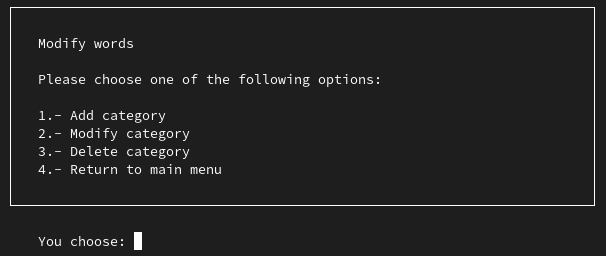
\includegraphics[width=0.7\linewidth]{img/modify_words}
				\caption{Menu to modify words}
				\label{fig:modifywords}
			\end{figure}
			
			\subsection{Add Category}
				Whenever a user chooses to add a category the program will show the categories that already exist in the file and will ask the user to enter the name of the new category.
				If the user inputs a category name that already exists the program will show an error.
				\begin{figure}[hbtp]
					\centering
					
\includegraphics[width=0.7\linewidth]{img/add_category}
					\caption{Adding a new category}
					\label{fig:addcategory}
				\end{figure}
			\subsection{Modify Category}
				If the user chooses this option the following menu will be shown:
				\begin{figure}[hbtp]
					\centering
					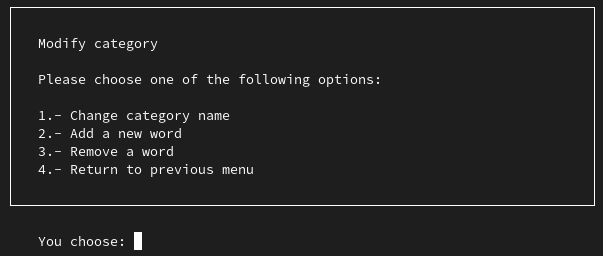
\includegraphics[width=0.7\linewidth]{img/modify_category}
					\caption{Modifying a category}
					\label{fig:modifycategory}
				\end{figure}
				On each of the options the user will first be asked which category they want to modify.
				
				For or removing words, once the user has entered the category name that the words belongs to, a list of words from that category will also be shown.
				\begin{figure}[hbtp]
					\centering
					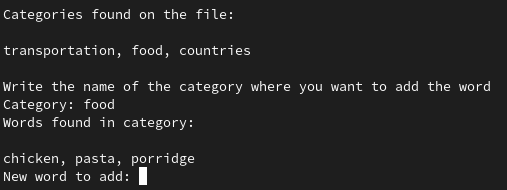
\includegraphics[width=0.7\linewidth]{img/add_word}
					\caption{Adding a new word}
					\label{fig:addword}
				\end{figure}
			
			\subsection{Delete Category}
				As with add category the program will show the user the categories that exist in the file and ask the user to enter the name of the category to delete.
				
		\section{Play Game}
			If a user chooses to play a round of hangman the program will ask if they want to use words belonging to a specific category or any word from any category.

			\begin{figure}[hbtp]
				\centering
				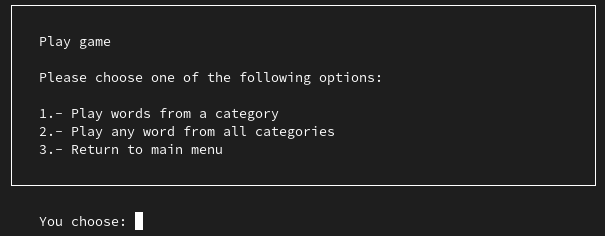
\includegraphics[width=0.7\linewidth]{img/play_game}
				\caption{Menu to start a new game}
				\label{fig:playgame}
			\end{figure}
		
			The game screen shows the number of lives left for the player and a picture of the hanged man. 
			The picture will change the more errors the player accrues.
			The screen will also show the length of the word in play by showing underscores for al the unknown letters.
			At the begging of the game all the letters will be unknown. 
			As the game progresses the letters will be uncovered.
			The game will also show the player the characters they have already tried, and prevent the usage of the same character more than once.
			
			Whenever the player enters a letter that is not in the word in play the game will show a message and it will subtract a life from the player.
			The game ends when the player has uncovered the hidden word, by guessing the individual letters or the whole word, or when the player has no more lives left.
			
			\begin{figure}[hbtp]
				\centering
				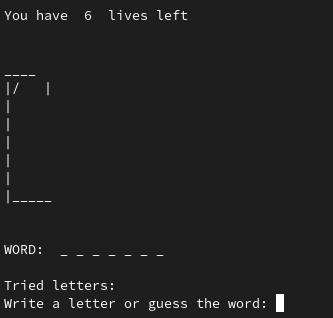
\includegraphics[width=0.7\linewidth]{img/game_start}
				\caption{Starting a new game}
				\label{fig:gamestart}
			\end{figure}
		
			\begin{figure}[hbtp]
				\centering
				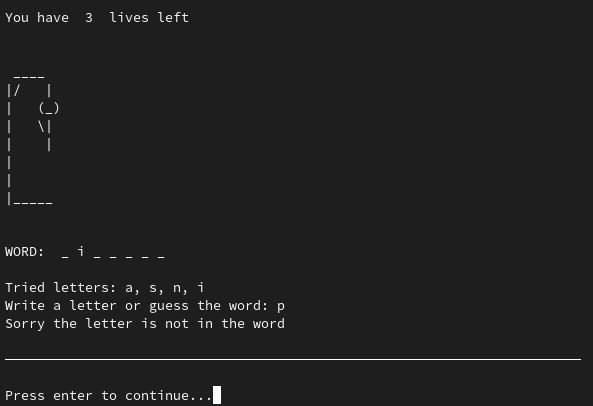
\includegraphics[width=0.7\linewidth]{img/game_error}
				\caption{The player has chosen a letter that is not in the word}
				\label{fig:gameerror}
			\end{figure}
		
			\begin{figure}[hbtp]
				\centering
				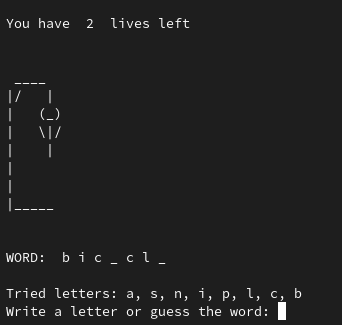
\includegraphics[width=0.7\linewidth]{img/game_advanced}
				\caption{An advanced stage of a game}
				\label{fig:gameadvanced}
			\end{figure}
		
			
			
\end{document}